\documentclass{article}
\usepackage{graphicx}
\usepackage{biblatex}
\usepackage[spanish]{babel}
\addbibresource{Practica04-Carrillo_Bonilla.bib}
\begin{document}
	\begin{titlepage}
		\centering
		\vfill
		\fbox{\Huge{Tercera práctica}} \\
		\vfill
		\large{\textsc{Hugo Tonatiuh Carrillo Bonilla}}\\
		\vfill
		320026379
		\vfill
		\begin{center}
			
\includegraphics[width=\linewidth]{./images/Portada.png}
		\end{center}
		\vfill
	\end{titlepage}
	\section*{Parte 1: Variables}
		\subsection*{Actividad 1.1 - Variables en Jshell}
			Escribiendo las variables una por una.
			\begin{center}
				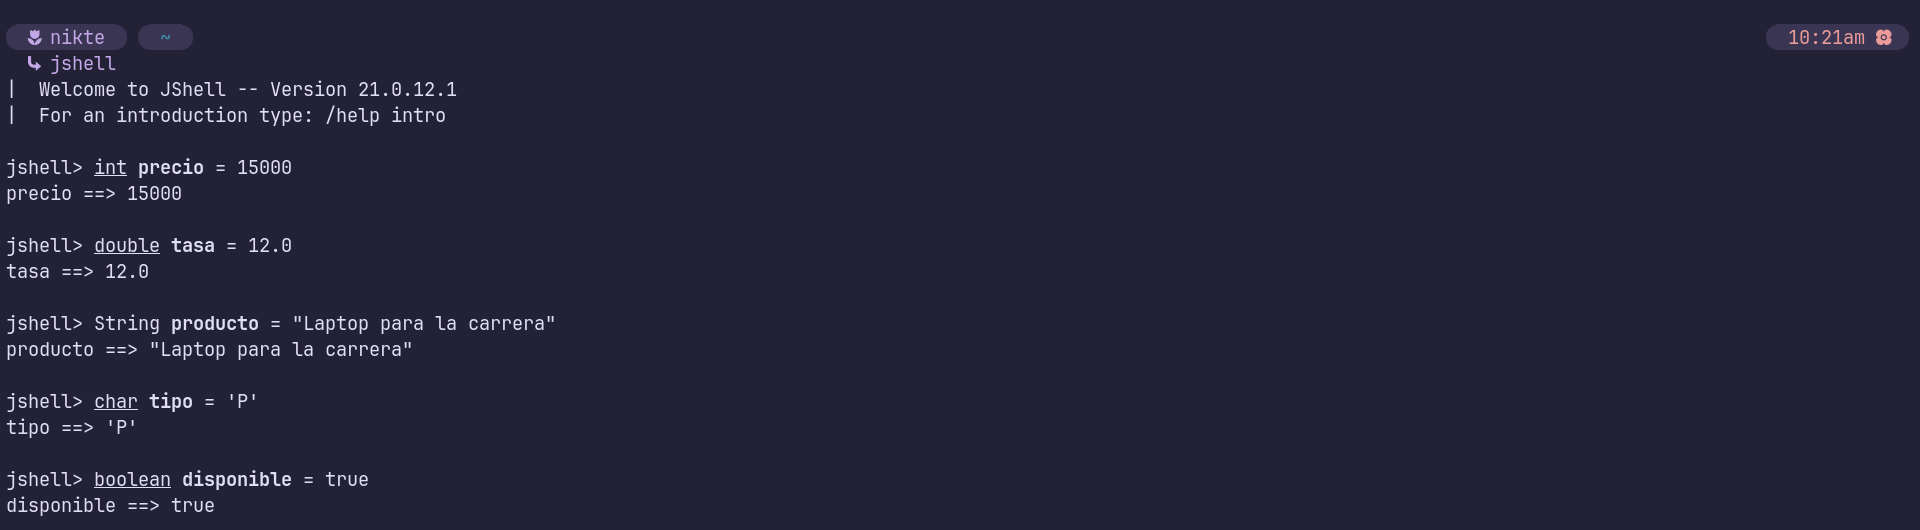
\includegraphics[width=\linewidth]{./images/P1-1-1.png}
			\end{center}
			Escribiendo únicamente el nombre de las variables.
			\begin{center}
				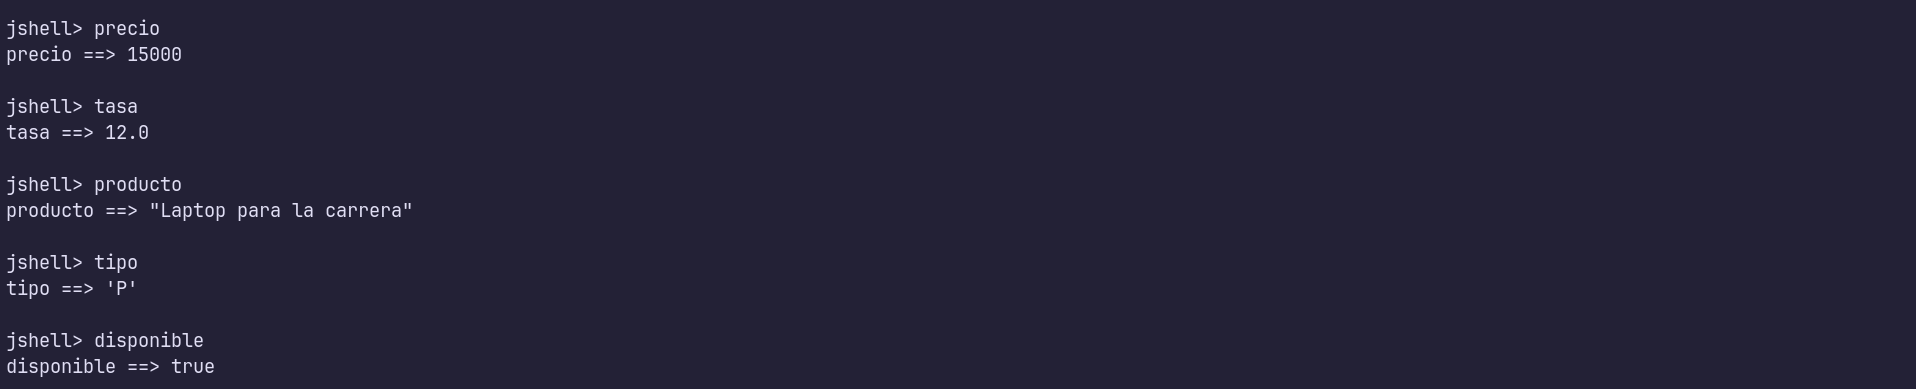
\includegraphics[width=\linewidth]{./images/P1-1-2.png}
			\end{center}
			Cambiando la variable \texttt{precio}.
			\begin{center}
				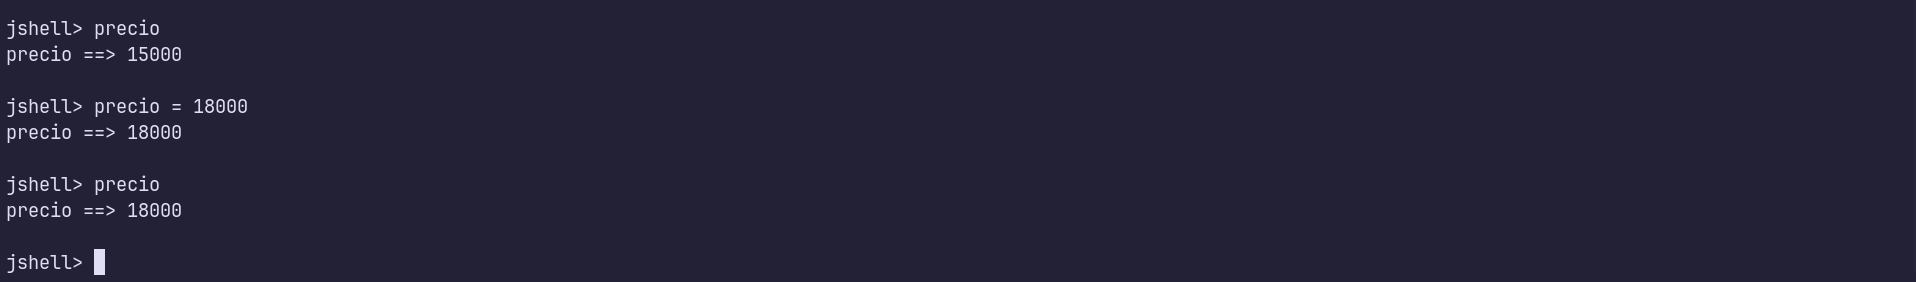
\includegraphics[width=\linewidth]{./images/P1-1-3.png}
			\end{center}
			Al principio, quise ver si \texttt{String} se comporta como un dato algebraico que puedes dividir y multiplicar como en lenguages elegantes y sofisticados. Después ví que se puede operar entre \texttt{int} y \texttt{float} sin relativamente ningún problema. Se pueden concatenar cadenas con números y además ví que \texttt{char} se comporta como un número. Sin embargo, \texttt{boolean} no admite valores que no sean estrictamente booleanos.
			\begin{center}
				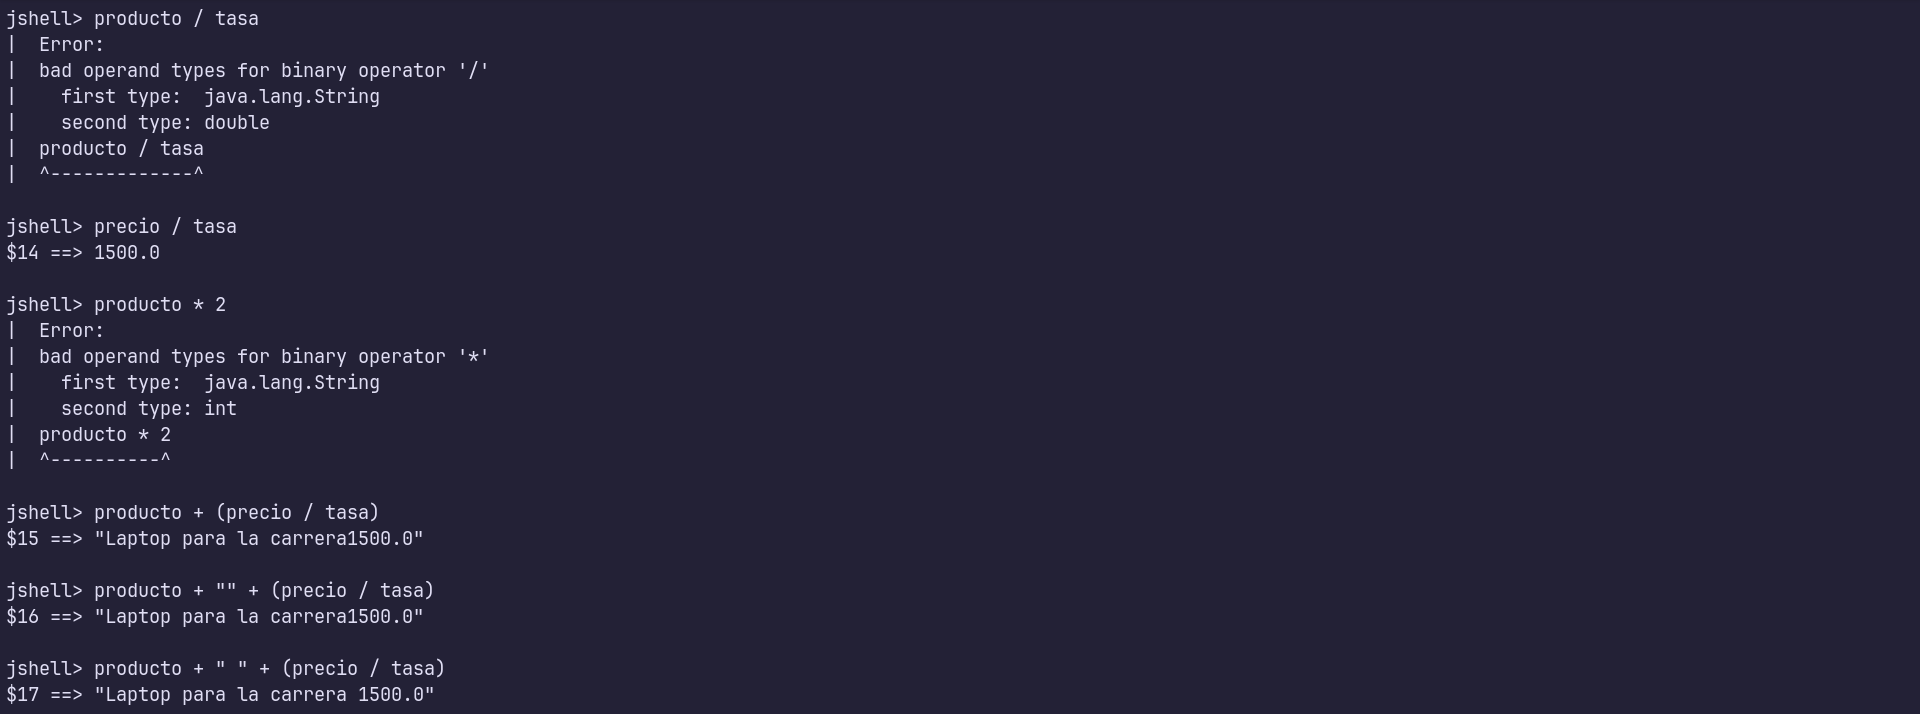
\includegraphics[width=\linewidth]{./images/P1-1-4.png}
			\end{center}
			\begin{center}
				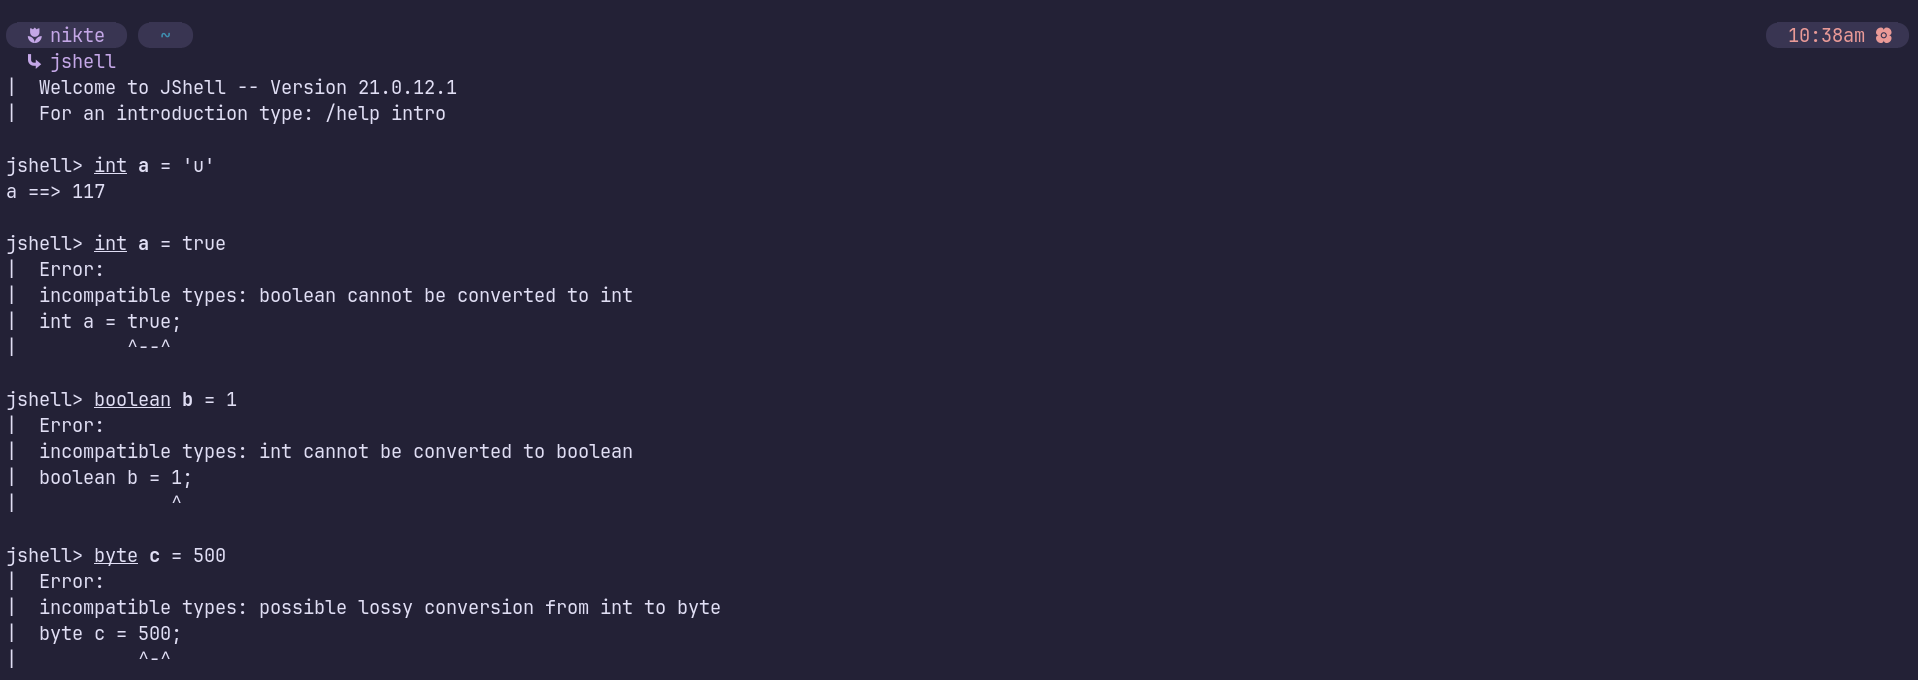
\includegraphics[width=\linewidth]{./images/P1-1-5.png}
			\end{center}
		\subsection*{Actividad 1.2 - Agregando variables en P2}
			Tuve que crear el archivo otra vez porque lo había borrado.
			\begin{center}
				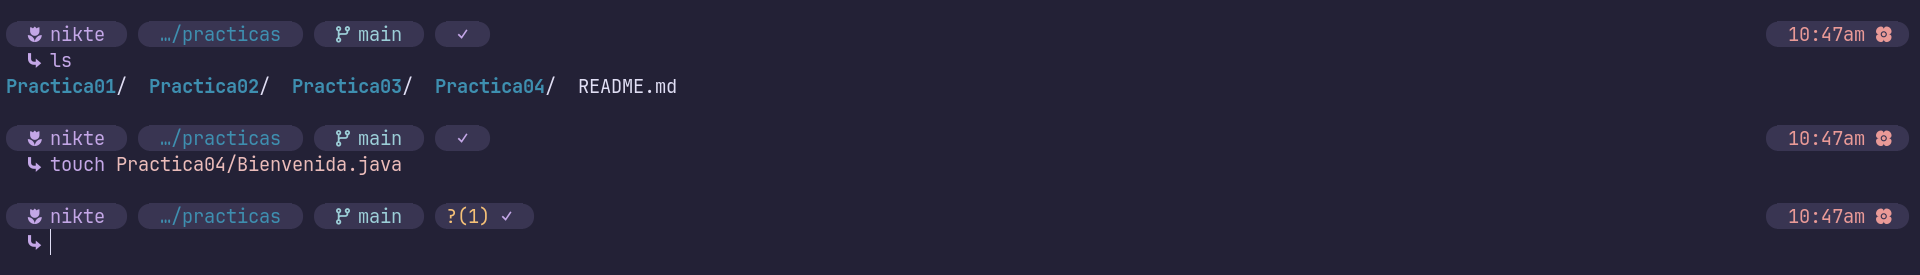
\includegraphics[width=\linewidth]{./images/P1-2-1.png}
			\end{center}
			Lo único elegante aquí fue lo que hice con \texttt{char}. Para los demás usé \texttt{String}. En el nombre la decisión me parece obvia. No así con el número de cuenta. En primera, no sé qué tipo de números de cuenta sean válidos, y por lo tanto puede ser que \texttt{int} no alcance. Además, sería peligroso dejar que el usuario manipule \textbf{numéricamente} esa información.
			\begin{center}
				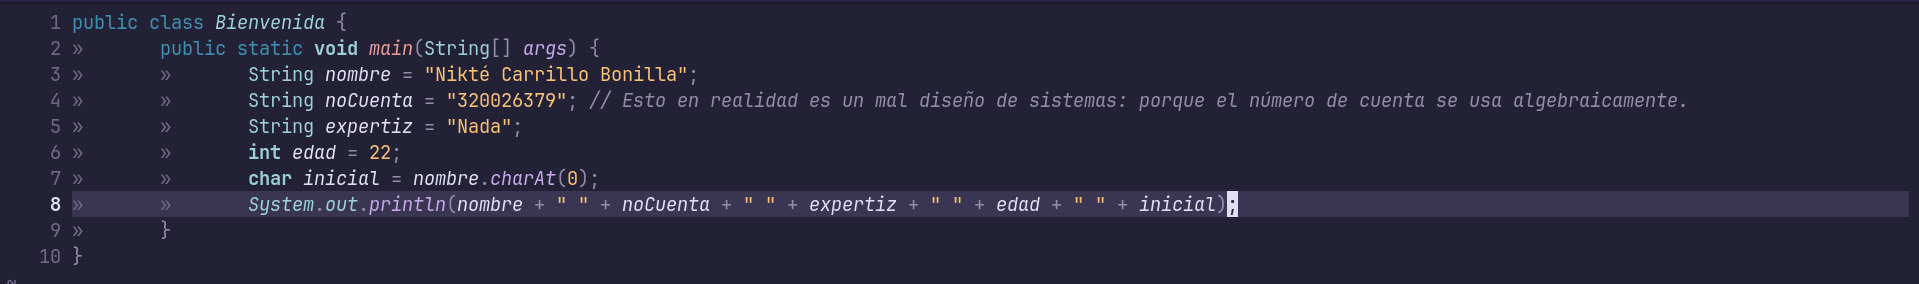
\includegraphics[width=\linewidth]{./images/P1-2-2.png}
			\end{center}
			El programa compiló sin problemas.
			\begin{center}
				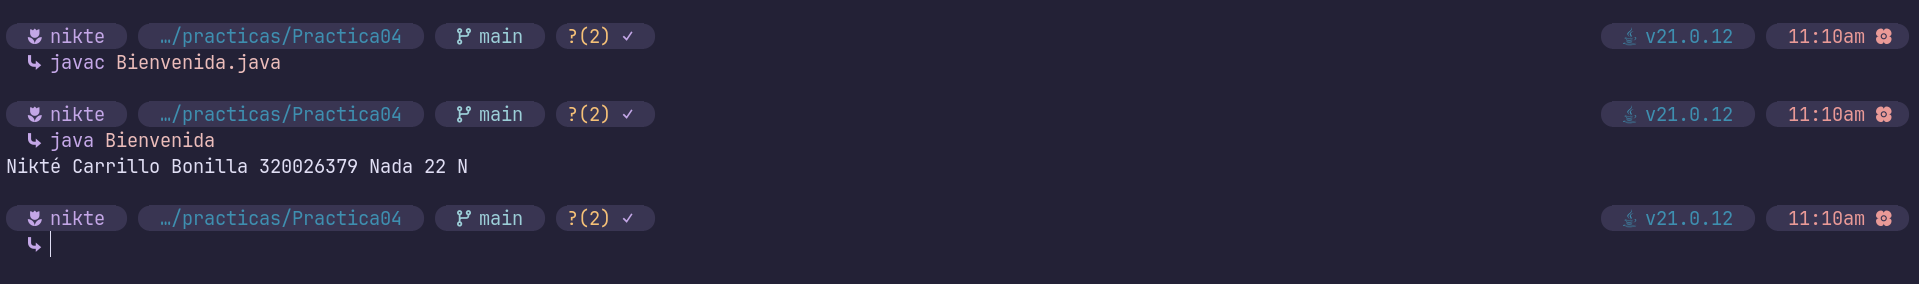
\includegraphics[width=\linewidth]{./images/P1-2-3.png}
			\end{center}
	\section*{Parte 2: Comentarios y expresiones elegantes}
		\subsection*{Actividad 2.1 - Comentarios en Java}
			También tuve que volver a descargar el programa \texttt{Programa.java}.
			\begin{center}
				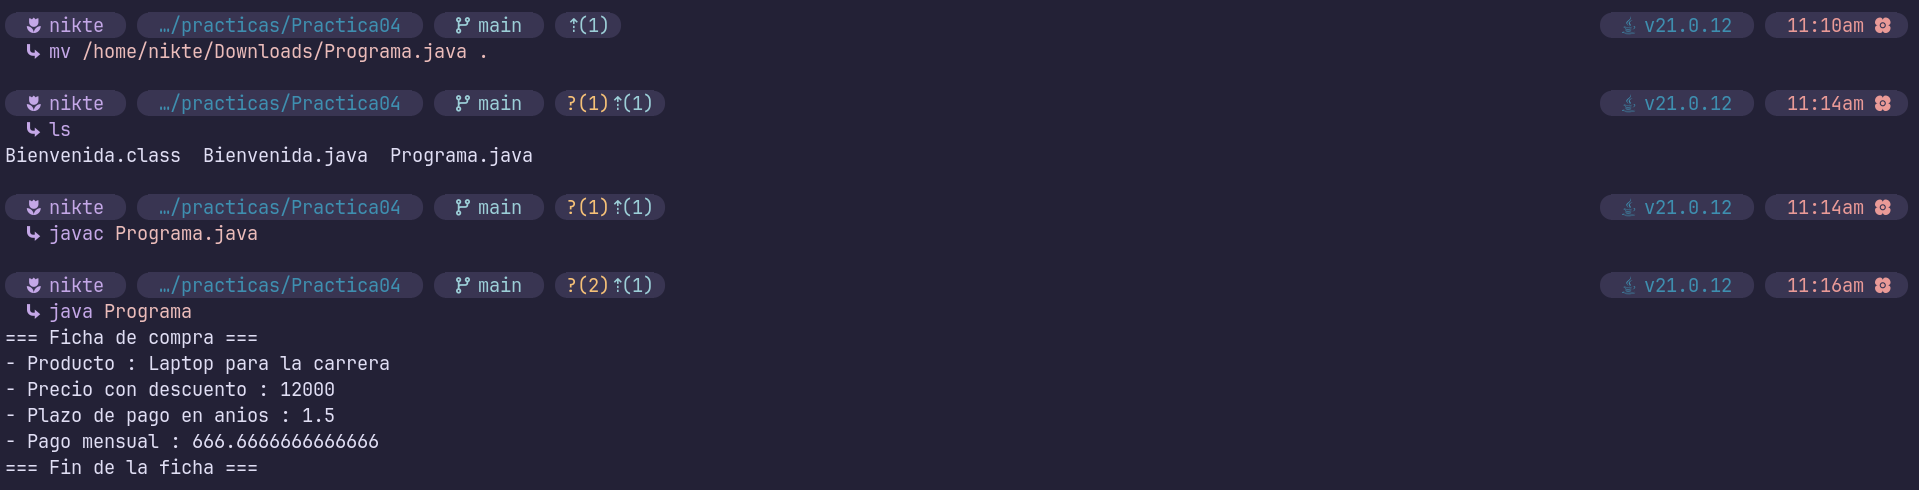
\includegraphics[width=\linewidth]{./images/P2-1-1.png}
			\end{center}
			Los comentarios que hice me parecen prudentes porque muchos de mis compañerxs tienen mucha curiosidad de qué es lo que pasa realmente con la firma del método principal.
			\begin{center}
				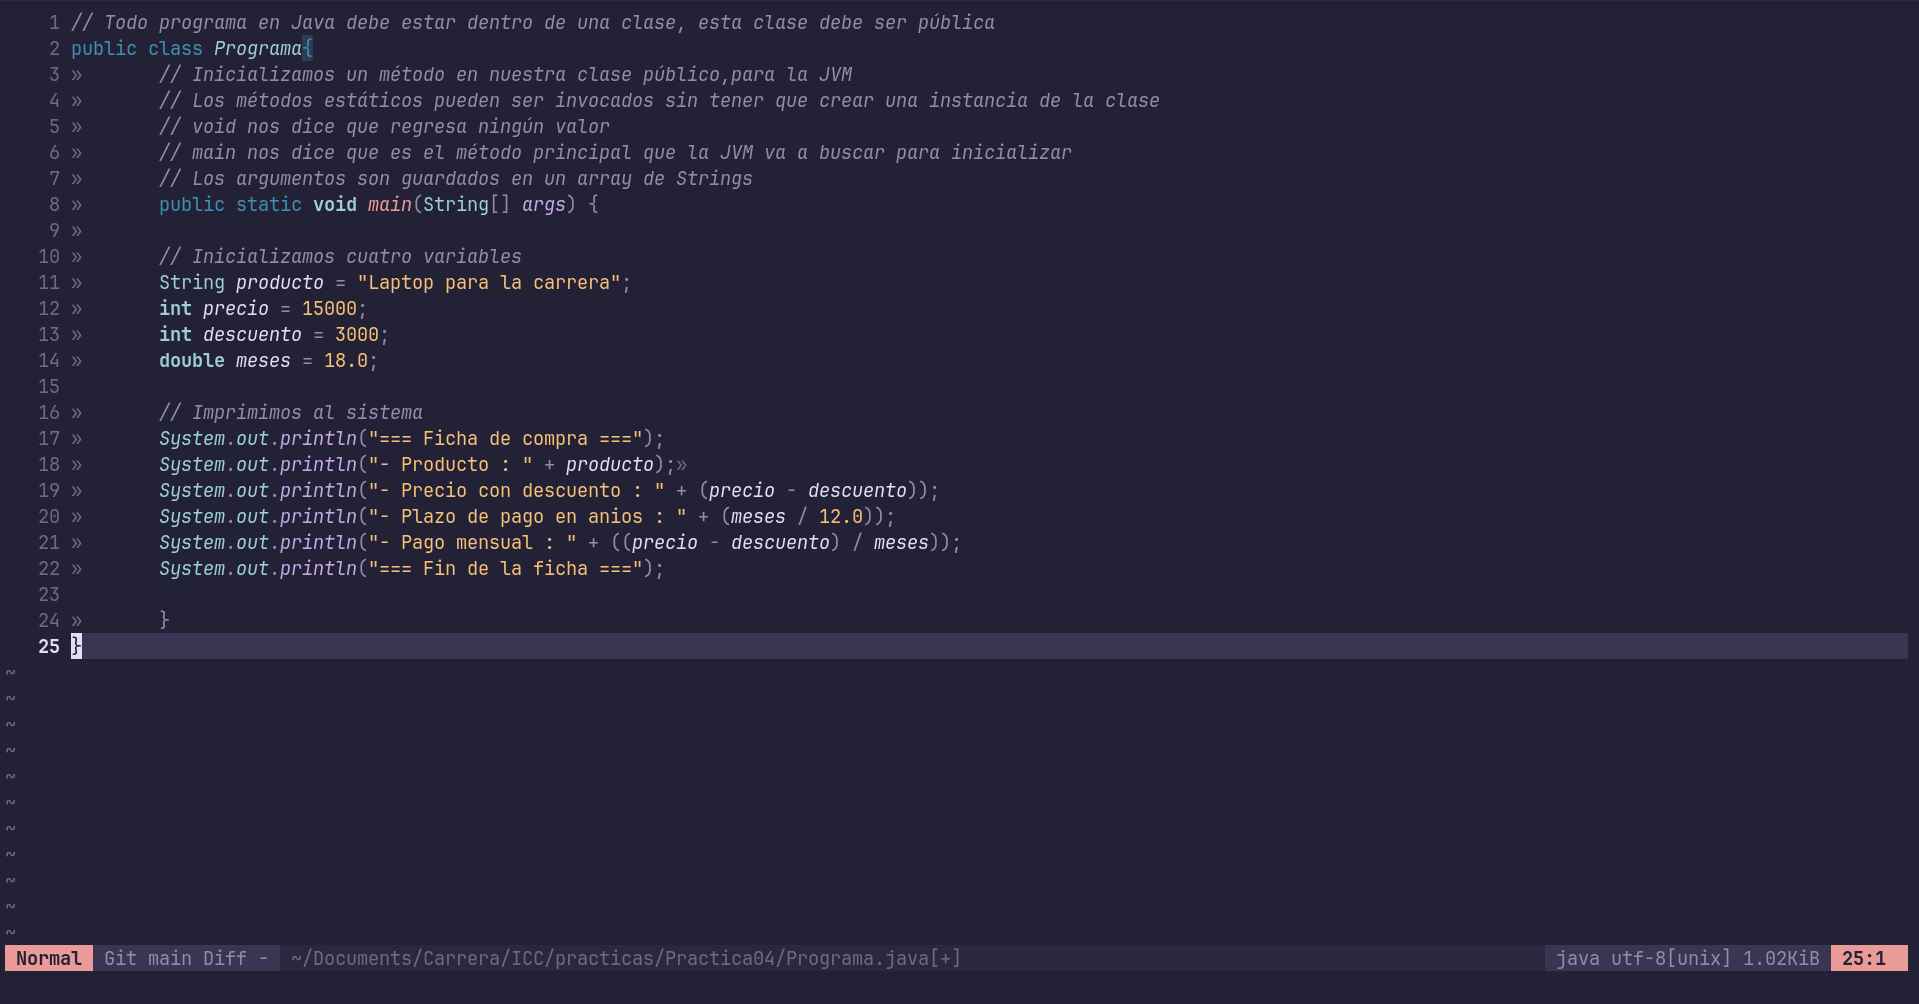
\includegraphics[width=\linewidth]{./images/P2-1-2.png}
			\end{center}
			Después de hacer comentarios, el programa sigue corriendo bien.
			\begin{center}
				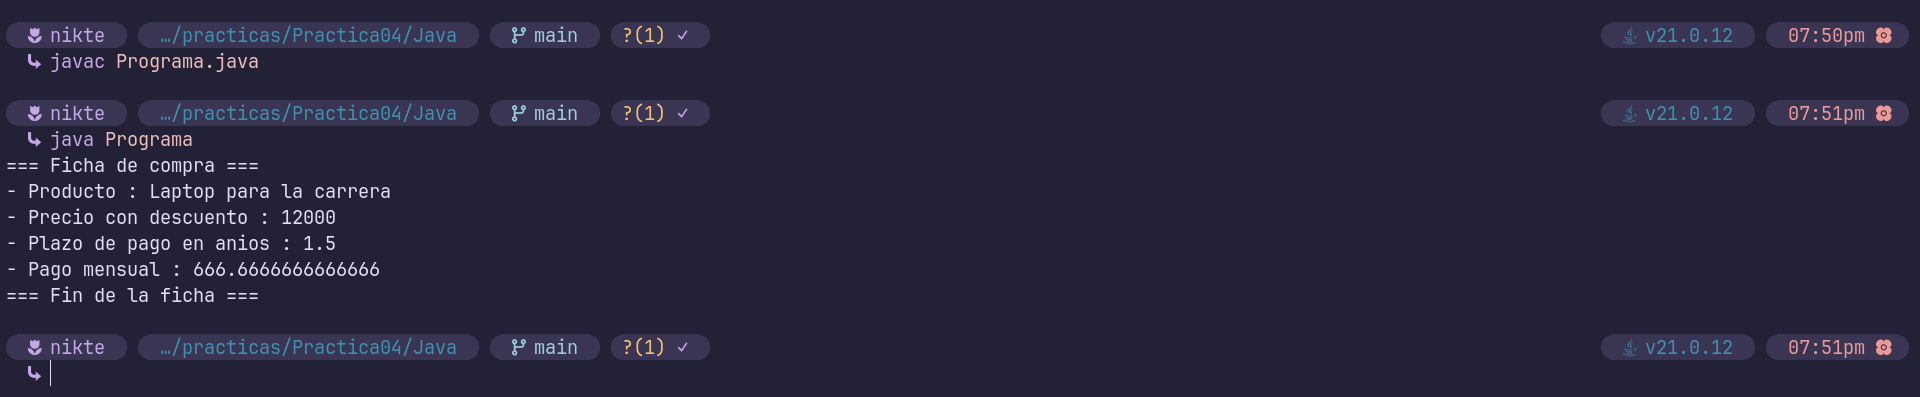
\includegraphics[width=\linewidth]{./images/P2-1-3.png}
			\end{center}
		\subsection*{Actividad 2.2 - Printf}
			Consulté una página de internet para resolver esta actividad \cite{printf}. \texttt{printf} utiliza placeholders precedidos con \% para distintos tipos de datos. Para \texttt{float}, podemos controlar el número de dígitos después del punto decimal con \texttt{\% .2f}.

			Renombré el archivo sin saber que también tenía que subir el archivo con comentarios.
			\begin{center}
				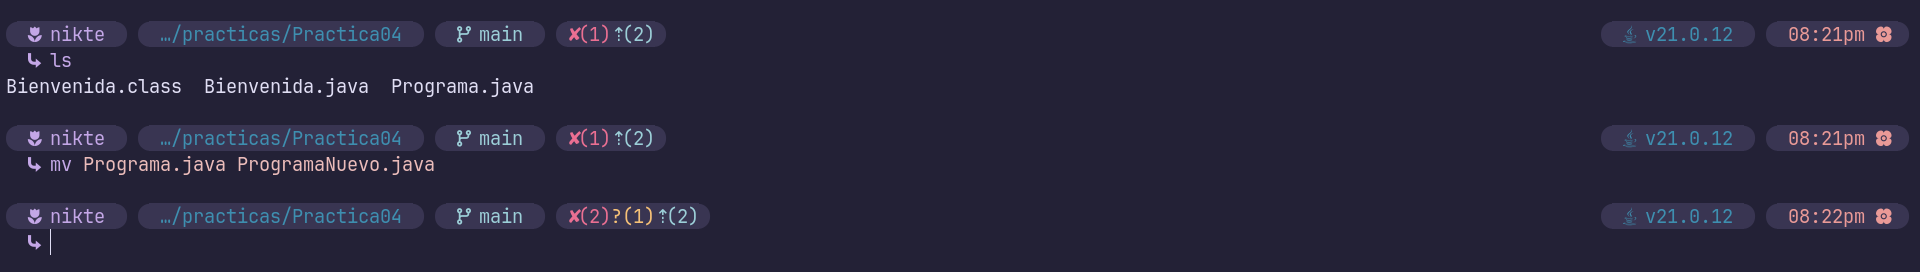
\includegraphics[width=\linewidth]{./images/P2-2-1.png}
			\end{center}

			Aquí formateo el output del programa solo para anios.
			\begin{center}
				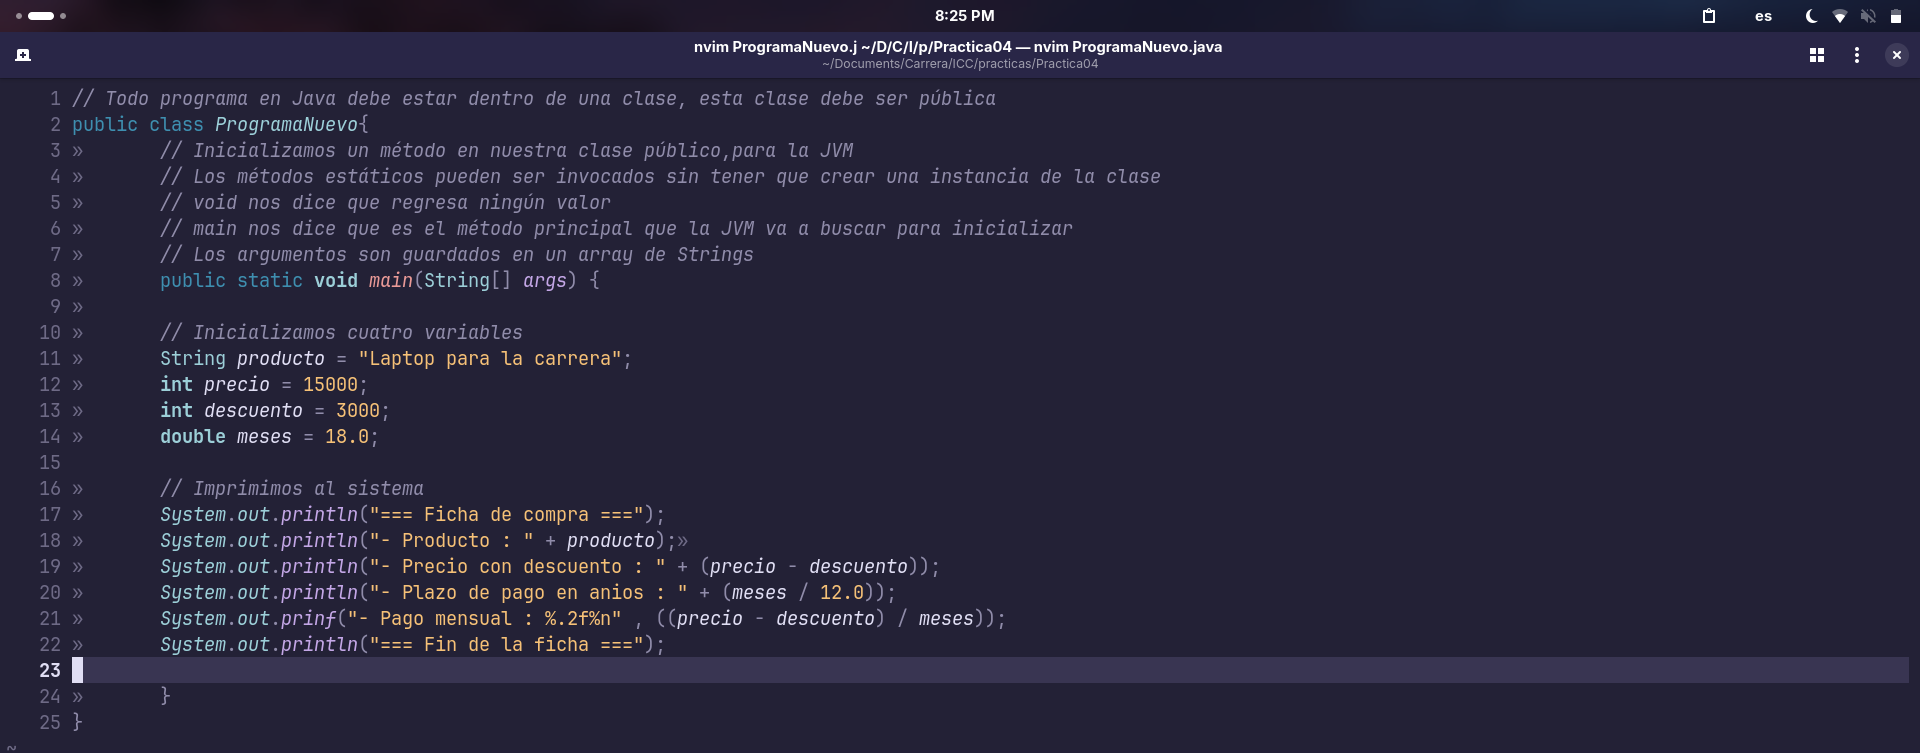
\includegraphics[width=\linewidth]{./images/P2-2-2.png}
			\end{center}

			Aquí formateo para que todo el output del programa se encuentre en una sola línea
			\begin{center}
				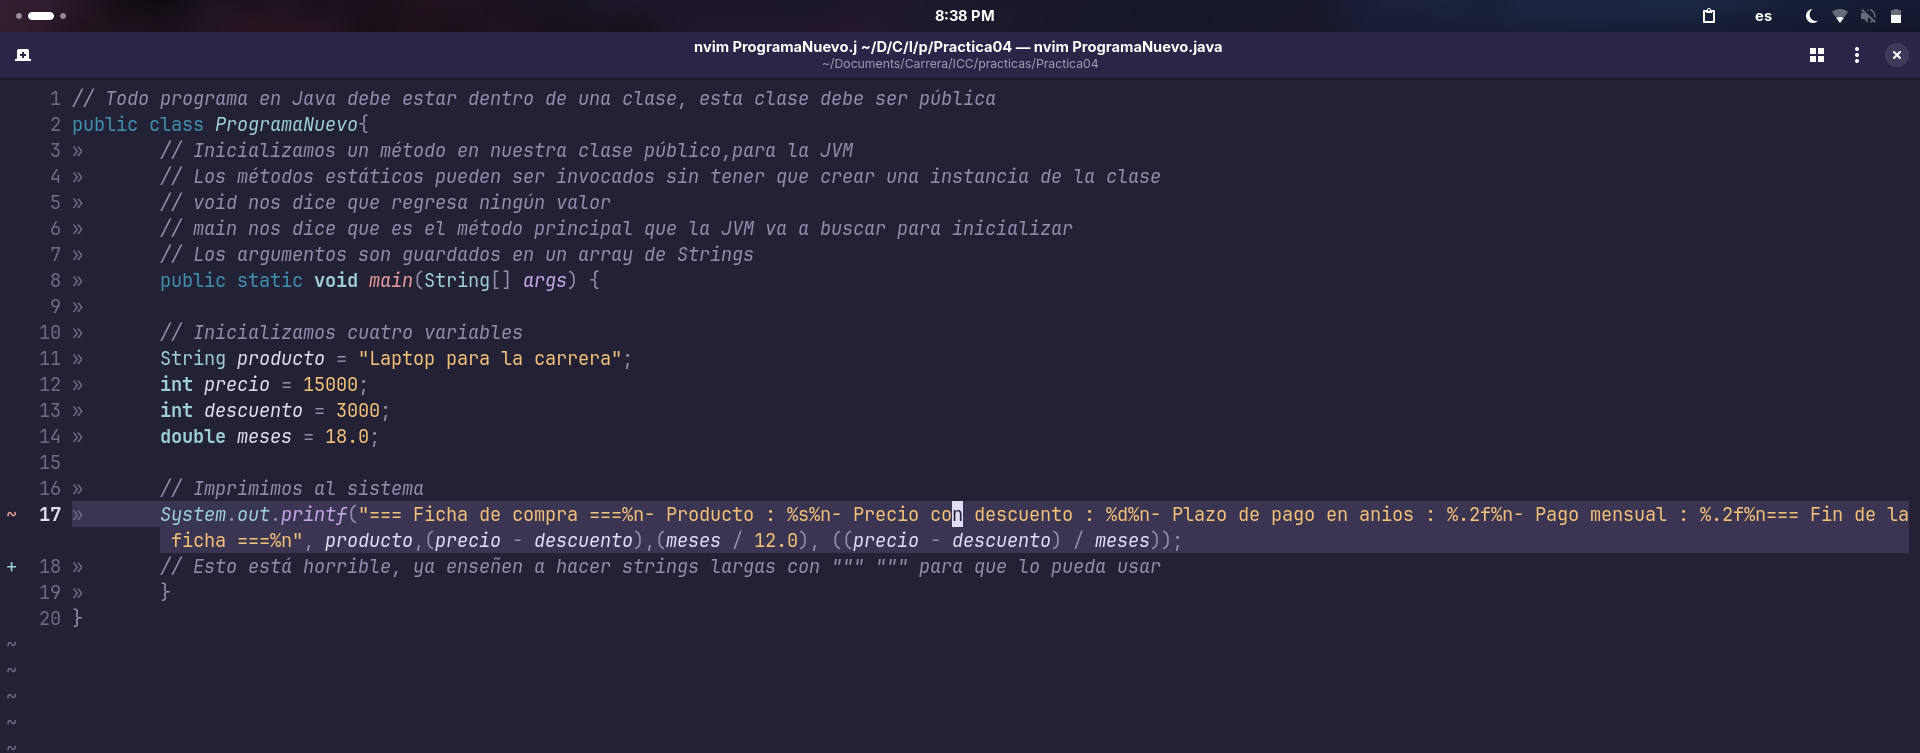
\includegraphics[width=\linewidth]{./images/P2-2-3.png}
			\end{center}

			El programa corre sin problemas.
			\begin{center}
				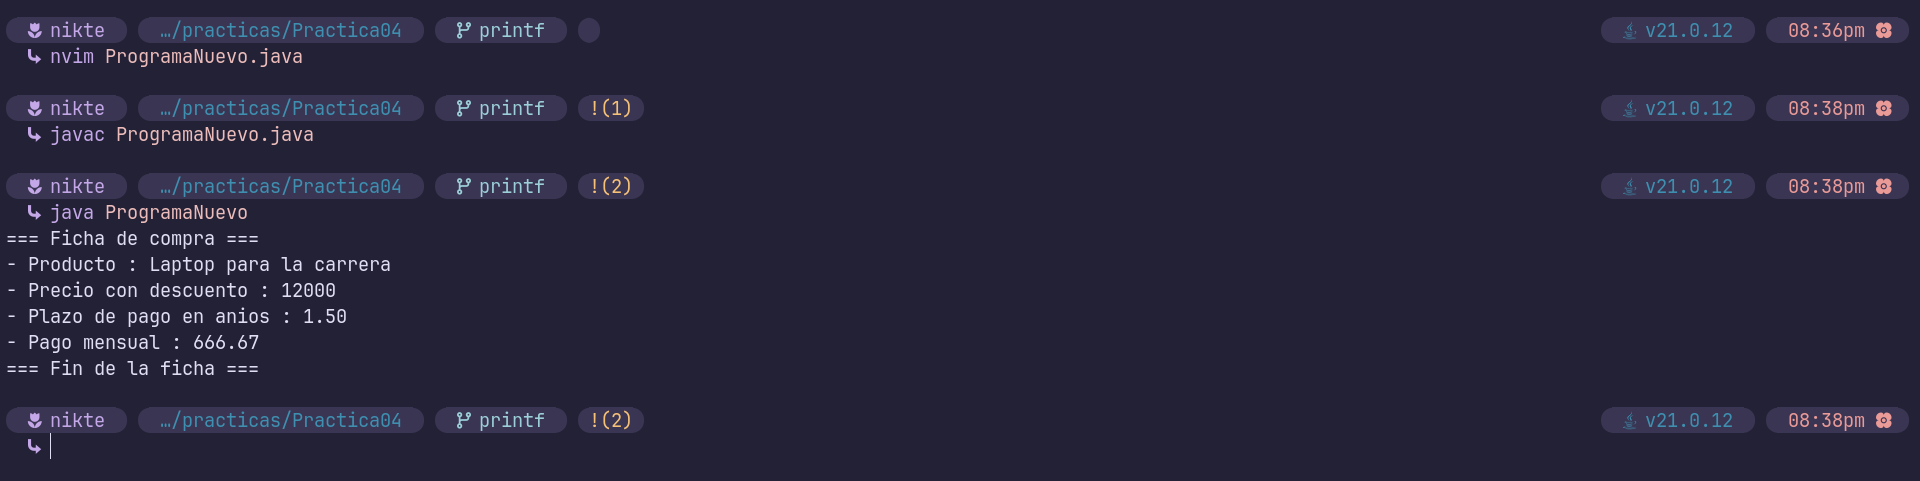
\includegraphics[width=\linewidth]{./images/P2-2-4.png}
			\end{center}
			\printbibliography
	\section*{Parte 3: Reto de abstracción}
		\subsection*{Actividad 3.1 - Filtrando información}
			He aquí una lista condensada de los datos que aprecié como necesarios y como innecesarios.
			\textbf{Datos necesarios:}
			\begin{itemize}
				\item Precio de la laptop.
				\item En concreto, el precio de la laptop de nuestro primer cliente
				\item La cantidad de mensualidades en las que van a pagar
				\item Interés anual del 15\% .
				\item Pago en total.
			\end{itemize}

			El precio es indispensable para saber cuánto cobraremos, en especial el de Robbie, por esta misma razón debemos de saber en cuántas mensualidades nos va a pagar y su interés. Técnicamente el pago total lo sabremos nosotrxs, y no es un dato que se nos dé, sino que lo tenemos que deducir con la información dada.

			\textbf{Datos innecesarios:}
			\begin{itemize}
				\item Especificaciones de la laptop.
				\item La calificación del cliente.
			\end{itemize}

			Las especificaciones de la laptop nos son indiferentes, el cliente --- Robbie --- nos va a pagar incluso si su laptop la comprara descompuesta. Y la calificación del cliente, aunque es importante, no es vital pues no sabemos todavía la forma en la que su calificación afectará sus mensualidades o su interés. 

			De lejos, el dato que más me costó clasificar fue precisamente el de la calificación del cliente, porque a la vez tanto es importante para el subsecuente desarrollo de nuestro programa, como nos es superfluo para el problema a mano. Implementarlo además excede nuestras capacidades técnicas --- requeriríamos hacer un objecto \texttt{cliente} con la calificación como atributo --- y eso complicaría innecesariamente nuestra base de código demasiado pronto en el ciclo de desarrollo.

		\subsection*{Actividad 3.2 - Cumpliendo los deseos del señor Pines}
			Mi implementación me parece sumamente mediocre y subpar. La falta de herramientas de control de flujo lleva inevitablemente a que calculemos nuestro interés en una sola entrega en lugar de calcularlo año por año.
			\begin{center}
				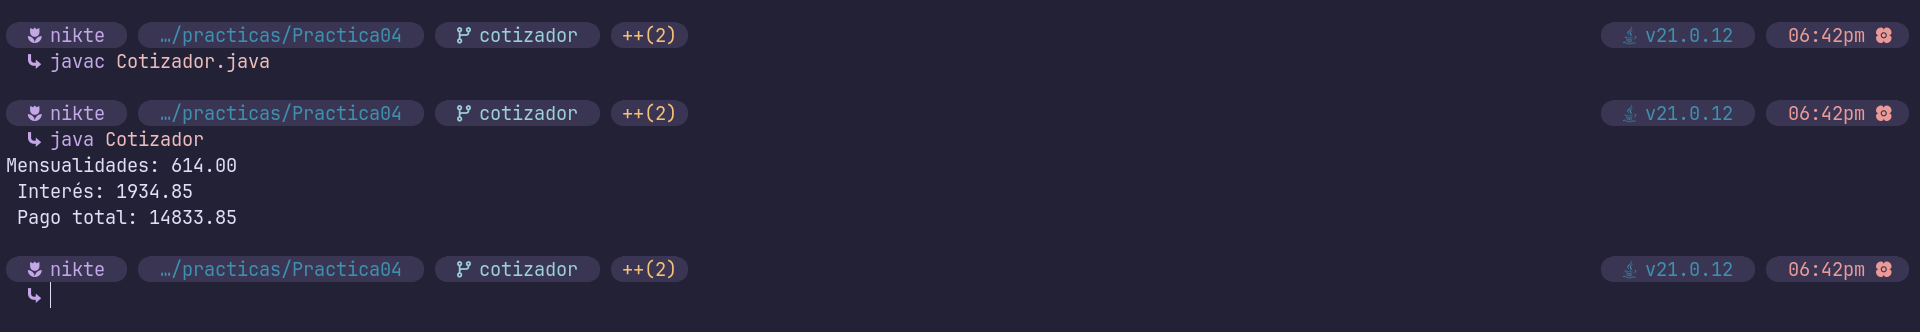
\includegraphics[width=\linewidth]{./images/P3-2-1.png}
			\end{center}
	\section*{Conclusión}
		Esta práctica es muy interesante porque por fin empezamos a resolver problemas de programación y es una gran motivación para empezar a aprender métodos tradicionales y procedurales de programación, como también nos deja atisbar la clase (ja, ja) de problemas que podremos resolver con objetos. Finalmente, pero no por ello menos importante, aprendí que debo empezar a leer con cuidado las instrucciones en general y los \textit{verbos} que se utilizan en particular, pues más de una vez tuve que realizar una tarea en múltiples ocasiones porque borraba, editaba y renombraba archivos que debía de dejar intactos.
\end{document}
